\documentclass[a4paper]{article}

\usepackage{pgfplots}

\pgfplotsset{compat=1.5}

\begin{document}


%\tracingmacros=2 \tracingcommands=2

\pgfplotsset{
	grid style={red},
	tick style={line width=5pt},
	axis background/.style={fill=yellow},
clip mode=individual,
}

\subsection*{This test uses \string\pgfplotssetlayers\space commands.}

\pgfplotssetlayers

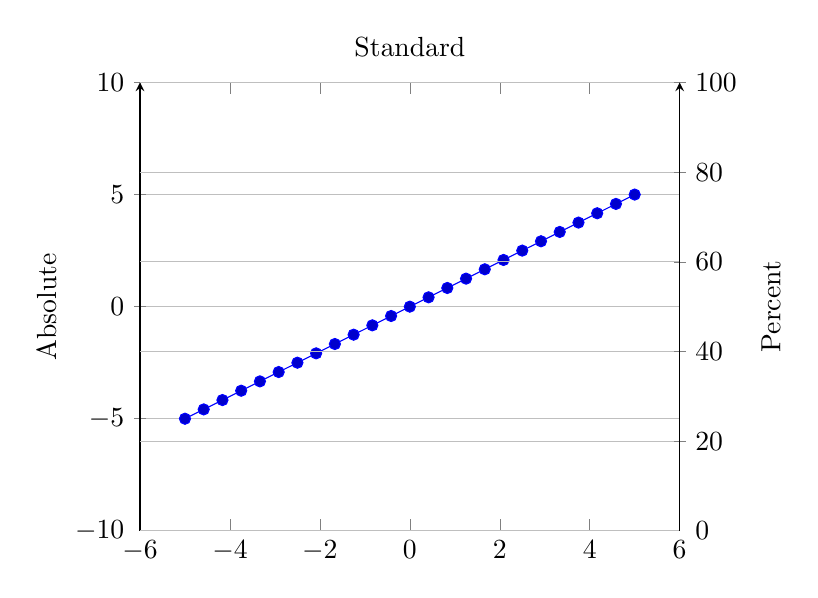
\begin{tikzpicture}
	\begin{axis}[ymin=-10,ymax=10,ylabel=Absolute,
		axis y line=left,
		ymajorgrids,
		title={Standard},
	]
		\addplot {x};
	\end{axis}

	\begin{axis}[ymin=0,ymax=100,
			xmin=0,xmax=1,% FIXME : optimize away!?
		axis x line=none,
		axis y line=right,
%		xshift=0.1cm,
		ylabel={Percent},
		ymajorgrids,
	]		
	\end{axis}
\end{tikzpicture}


\pgfplotssetlayers{axis on top}
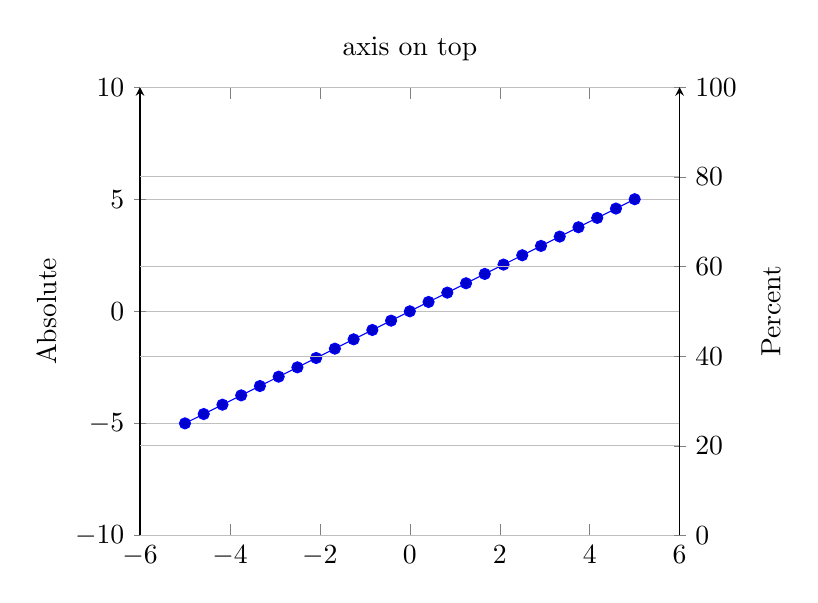
\begin{tikzpicture}
	\begin{axis}[ymin=-10,ymax=10,ylabel=Absolute,
		axis y line=left,
		ymajorgrids,
		title={axis on top},
	]
		\addplot {x};
	\end{axis}

	\begin{axis}[ymin=0,ymax=100,
			xmin=0,xmax=1,% FIXME : optimize away!?
		axis x line=none,
		axis y line=right,
%		xshift=0.1cm,
		ylabel={Percent},
		ymajorgrids,
	]		
	\end{axis}
\end{tikzpicture}

\pgfplotssetlayers{none}

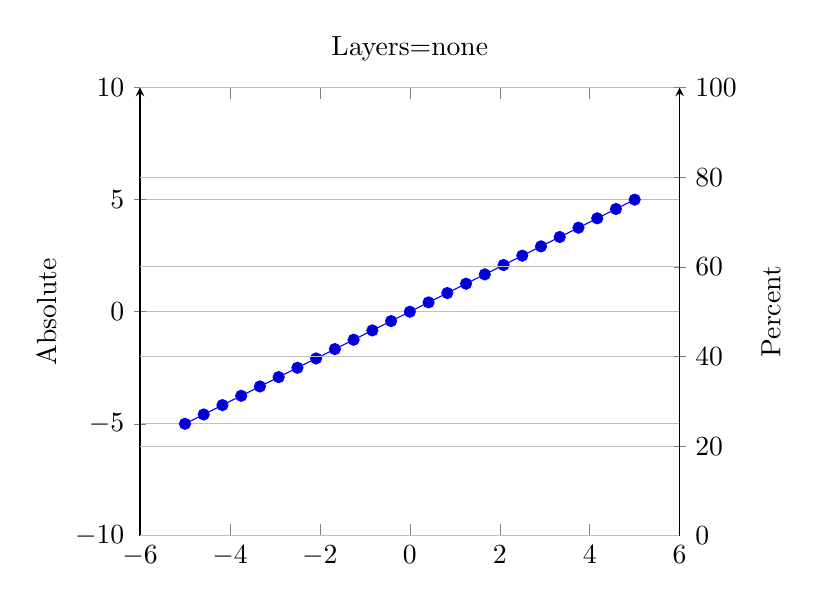
\begin{tikzpicture}
	\begin{axis}[ymin=-10,ymax=10,ylabel=Absolute,
		axis y line=left,
		ymajorgrids,
		title={Layers=none},
	]
		\addplot {x};
	\end{axis}

	\begin{axis}[ymin=0,ymax=100,
			xmin=0,xmax=1,% FIXME : optimize away!?
		axis x line=none,
		axis y line=right,
%		xshift=0.1cm,
		ylabel={Percent},
		ymajorgrids,
	]		
	\end{axis}
\end{tikzpicture}
\end{document}

